%Chapter 7

% Chapter 7 from the standard thesis template
% Conclusions and Future work
\chapter{CONCLUSION AND FUTURE WORK} \label{ch:conclusion}

\section{Conclusion}
In this thesis we have shown that an off the shelf SDR can be used to perform as a radiometer.  Using a SDR has several advantages such as a more flexible system and can result in a less expensive system by using commercial off the shelf components.  Since a SDR offers high flexibility, changes to the system can be done very quickly and helps in future proofing the system.

\section{Future work}\label{Futurework}

The work in this thesis demonstrated a basic radiometer system.  There are other more complex radiometer systems that can be implemented in software. These include a correlating radiometer or a Dicke radiometer that can improve stability of the radiometer without the need of additional equipment such as thermal electric coolers.   


\subsection{Improvements}
Several improvements can be done to further enhance this software defined radiometer.  One improvement is to remove the personal computer (PC) and move the software defined radio to a Field Programmable Gate Array (FPGA) or an Application Specific Integrated Circuit (ASIC) solution.  A second improvment is to reduce the dependcy on stable Low Noise Amplifiers (LNAs) by being able to compensate for instabilities in the system.  

\emph{Removing the PC.}  For this thesis we focused on the software that would run on a PC or comparable computer system running a full operating system like Linux.  This aids speeding up development by using software tools such as GNURadio to rapidly develop the software used to create a radiometer in software.  While this works just fine for testing the theory on an off the shelf SDR acting as a radiometer, it does require hardware that is capable of running a full operating system and the associated software.  For some applications of a radiometer, this is not a huge concern.  In the case for the ISU radiometer, the concern is not that large since the radiometer is not designed to be portable and requires additional support equipment such as a generator anyway.  However, other remote sensing applications, such as space based applications, would require a more efficient method.  It is very possible to move the software generated in GNURadio into the firmware of the N200.  This will help to offload the work needed by the computer and would allow for the computer or similar system to act as more of a control method and for data storage.  

\emph{Improving stability.}  One of the largest challenges with a radiometer is improving the stability of the radiometer.  Drifts in temperature can greatly affect the gains from the LNAs and also change how much noise all components in the radiometer contribute.  A software defined radio can help as we are digitizing the signal as soon as possible.  This helps in eliminating the analog components for power detection and even for filtering, but does not eliminate all physical hardware, mainly the LNAs.  In this thesis, we did not focus on this issue since the tests were done in a controlled lab environment.

However, a more compact, lower cost and easier setup would be to just have the LNAs attach directly to the SDR without any temperature compensation.  While this can be done, we have now lost stability in the LNAs and we need to compensate for that.  Several methods have been discussed to handle instability in a traditional radiometer.  Some of these methods would be suitable for implementation in a software defined radiometer.

A very traditional method is a Dicke radiometer.  A Dicke radiometer switches between the antenna and a known noise source.  A future work for a software defined radiometer would be to use a digitally generated noise source, such as a Gaussian noise source, and then switch between the antenna and this known noise source.  This noise source can also be adjusted and is performed in software, therefore stability in the noise source is not an issue.  

%One method that is discussed by William Goggins is to use a feedback loop to continuously adjust a variable attenuator [\cite{Goggins}].  In Goggins paper, he discusses using a servo that mechanically controls the attenuator.  However, since we are in the digital domain, we can control this all in software, and doing a feedback loop is quite easy for a computer to do.  

%Another method uses multiple temperature points that can be referenced at any time.  By using two known temperature references, we can quickly calibrate the radiometer[\cite{Hach}].  
 
\emph{Correlation.}  Another method to improve stability and sensitivity is to correlate the information with another input which can be another antenna looking at the same source or can be two polarization from the same antenna[\cite{Clapp}][\cite{Aitken}].  This results in two receiver systems looking at the same source and you have two signals, $S_1$ and $S_2$.  Since we are looking at the same source, both signals will be correlated in time, and when multiplied they will provide an output proportional to the strength of the source signal.  The noise introduced by each receiver will then have a lower correlation due to the random nature of the noise.  This results in a radiometer with a greater sensitivity due to the reduction of the noise even though two receivers are used [\cite{Fujimoto}].

The N200 software defined radio was chosen as it is capable of having two different daughter-cards plugged in.  Therefore, it is possible to have both sources enter the software defined radio and once digitized we can sum the magnitudes of the two incoming sources.  This is quite easy to do and is shown in figure \ref{correlating_sdr}.

{\begin{figure}[h!tb] 
\centering
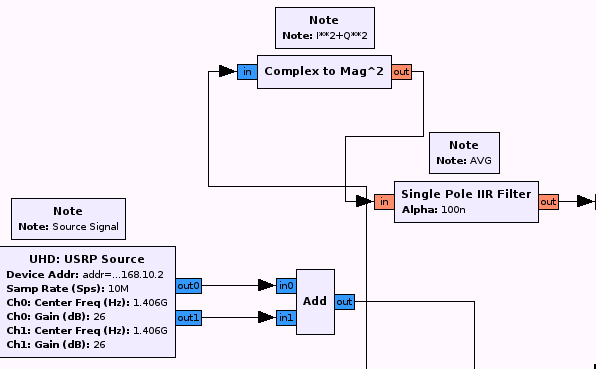
\includegraphics[width=14cm]{Images/N200_rad_corr.png}
\isucaption{The key blocks used for creating a correlating radiometer in software.  The key blocks is the USRP source, which allows us to address both daughter-boards and the ADD block which sums the signals.}
\label{correlating_sdr}
\end{figure}
}

Although figure \ref{correlating_sdr} shows a correlating software defined radio radiometer, it has not been tested.  In theory, this should correlate the signal and improve the sensitivity of the radiometer, however further testing is needed.

\subsection{Further testing}
The improvements and additional features outlined in Section \ref{Futurework} will require additional testing and verification.  While it has been shown that a software defined radiometer operates identically to a traditional radiometer, further testing is needed to verify different operating modes of a software defined radiometer.

\section{Closing statement}
This thesis demonstrated that it is possible to use off the shelf components and a software defined radio to implement a working radiometer that can be used in various radiometer applications such as soil moisture, ocean salinity and radio astronomy.  Use of a software defined radiometer can potentially allow radiometers to be used by a wider audience of users by creating an easy to user GUI and reducing the cost and hardware complexity that most radiometers require.  The result is more locations that are able to use radiometers as remote sensing tools to learn more about our planet and even the cosmos.
%----------------------------------------------------------
% End of Chapter 7.  Anything below this is extra information